\documentclass{book}
\usepackage[utf8]{inputenc}
\usepackage{pgfplots}
\pgfplotsset{compat=1.15}
\usepackage{mathrsfs}
\usetikzlibrary{arrows}
\usepackage{amsmath}
\usepackage{tikz}
\usepackage{wrapfig}
\usepackage{parskip}
\usepackage[most]{tcolorbox}
\usepackage{amssymb}
\usepackage{amsthm}
\usepackage[margin=0.7in]{geometry}
\usepackage{mathtools}
\usepackage{caption}
\usepackage{float}
\usepackage{enumitem}

\newtheorem{theorem}{Theorem}
\newtheorem{definition}[theorem]{Definition}
\newtheorem{claim}[theorem]{Claim}
\newtheorem{proposition}[theorem]{Proposition}
\newtheorem{lemma}[theorem]{Lemma}
\newtheorem{corollary}[theorem]{Corollary}
\newtheorem{conjecture}[theorem]{Conjecture}
\newtheorem*{observation}{Observation}
\newtheorem*{example}{Example}
\newtheorem*{remark}{Remark}

\usepackage{physics}
\usepackage{amsmath}
\usepackage{tikz}
\usepackage{mathdots}
\usepackage{yhmath}
\usepackage{cancel}
\usepackage{color}
\usepackage{siunitx}
\usepackage{array}
\usepackage{multirow}
\usepackage{amssymb}
\usepackage{gensymb}
\usepackage{tabularx}
\usepackage{extarrows}
\usepackage{booktabs}
\usetikzlibrary{fadings}
\usetikzlibrary{patterns}
\usetikzlibrary{shadows.blur}
\usetikzlibrary{shapes}




\tcbset{mytitle/.style={title={Question~\thetcbcounter\ifstrempty{#1}{}{: #1}}}}
\newtcolorbox[auto counter, number within=chapter, number freestyle={\noexpand\thechapter.\noexpand\arabic{\tcbcounter}}]{question}[1][]{%
    enhanced,
    breakable,
    fonttitle=\bfseries,
    mytitle={},
    #1
}


\title{Solutions to A course in combinatorics by J.H.van Lint \& R.M.Wilson}
\author{Aakash Ghosh }
\begin{document}
\maketitle
\tableofcontents

\chapter{Graphs}
\textit{Terminology of graphs and digraphs, Eulerian circuits, Hamiltonian circuits}\\
\textbf{Problem 1A} (i) Show that the drawings in Fig. 1.1 represent the
same graph (or isomorphic graphs).\\
(ii) Find the group of automorphisms of the graph in Fig. 1.1.\\
Remark: There is no quick or easy way to do this unless you are
lucky; you will have to experiment and try things.
\begin{center}
    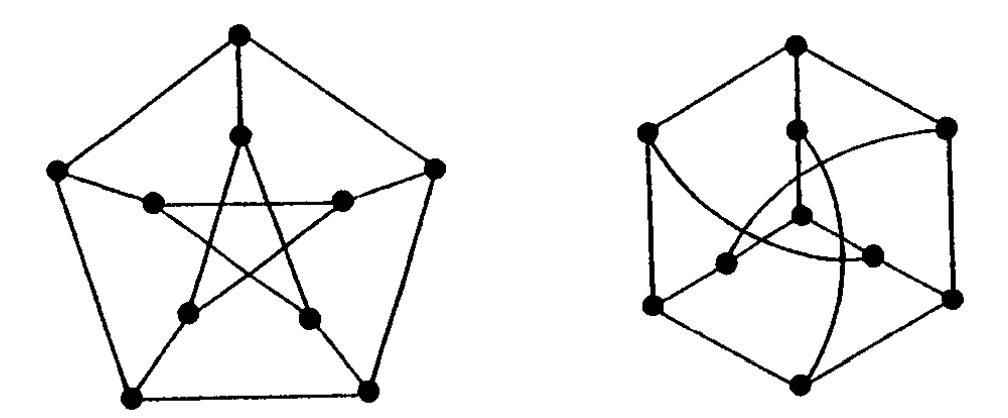
\includegraphics[width=0.7\textwidth]{Fig1.png}
\end{center}
\textbf{Solution 1A}\\
(i) This graph is know as the peterson graph. Label each vertex as 2 element subsets of $\{1,2,3,4,5\}$. Two vertex is connected by an edge if and only if they are disjoint. The corresponding labeling are shown below. 
\begin{center}
    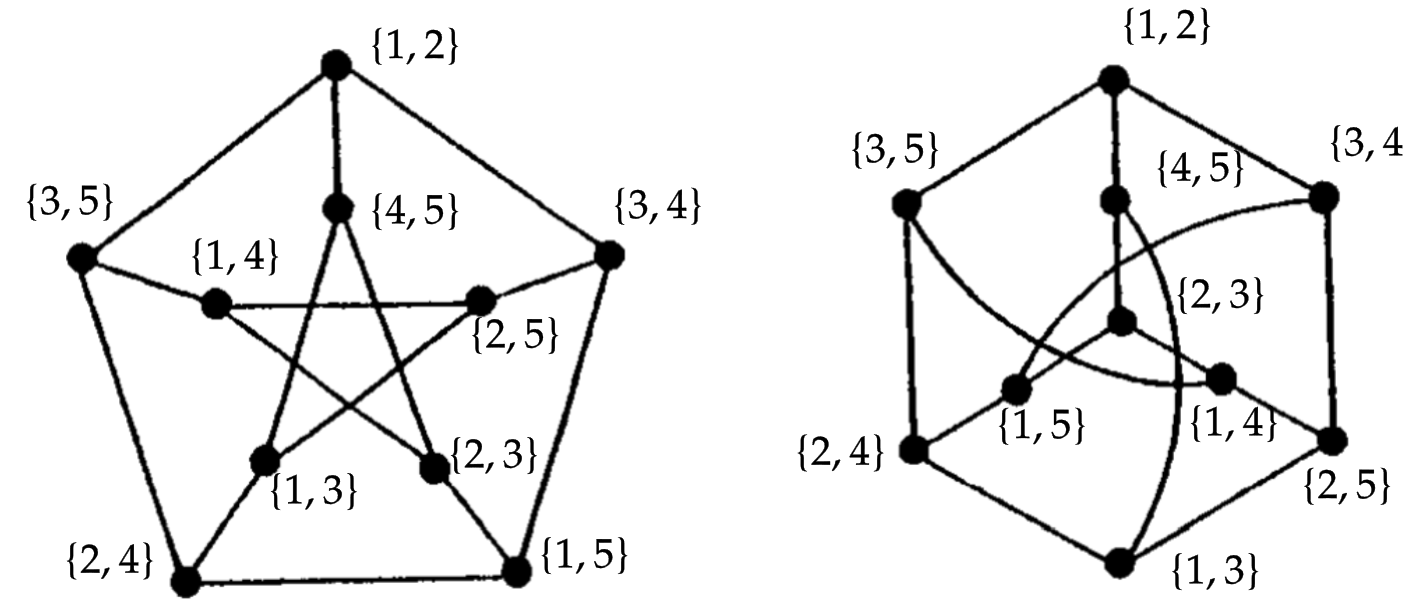
\includegraphics[width=0.7\textwidth]{Fig 2.png}
\end{center}
(ii) It follows that the automorphisms of this graph is precisely the permutations of $\{1,2,3,4,5\}$\\\\
\textbf{Problem 1B} Suppose $G$ is a simple graph on 10 vertices that is
not connected. Prove that $G$ has at most 36 edges. Can equality
occur?\\
\textbf{Solution 1B}\\
Let $G$ be the disconnected graph with maximum edges. Then $G$ has atleast 2 disconnected components. We can assume each component is complete as adding edges within a component doesn't destroy disconectivity. Furthermore, we can assume that there are exactly 2 disconnected components (If there are more than 2 components $G_1,G_2\hdots G_n$ then we can increase the number of edges by joining all vertices between $G_i$ and $G_j$ where $i,j\ne 1$. As $G_1$ stays disconnected from the rest, the end graph is disconnected). Let the disconnected components have $v_1$ and $v_2$ vertices with $v_1\leq v_2$. We claim that $v_1=1$. If not, then  $v_1>1$. Pick an edge from $G_1$(complete graph induced by $v_1$ vertices) and move it to $G_2$(complete graph induced by $v_2$ vertices). $G_1$ loses $v_1-1$ edges and $G_2$ gains $v_2$ edges. As $v_2\geq v_1$, $v_2-v_1+1>0$ which contradicts the fact that $G$ has the maximum number of edges possible. Therefore, $v_1=1$ and $v_2=9$. It follows that $G$ is formed by a single vertex and a $K_9$ and has a total of ${9\choose 2}=36$ edges.     \\\\
\textbf{Problem 1C} Show that a connected graph on $n$ vertices is a tree
if and only if it has $n - 1$ edges.\\
\textbf{Solution 1C}
Let $G$ be connected with $n-1$ edges. We  show $G$ is a tree. This is true for graphs with $n=2$ vertices. Assume this is true for a graph with $|G|\leq n$ vertices. Consider a tree with $n+1$ vertices. Remove an edge. Then the graph is converted to two disjoint trees: this is because if removing an edge $\{v_i,v_j\}$
doesn't make the graph disjoint then there exists simple a paths between $v_i$ and $v_j$ other than $\{v_i,v_j\}$ and therefore a cycle exists. The absence of cycles is trivial as there were no cycles to begin with. Let the two trees have $v_1$ and $v_2$ vertices. Then by our induction hypothesis, they have $v_1-1$ and $v_2-1$ edges respectively. Therefore $G$ has $v_1-1+v_2-1+1=v_1+v_2-1=n$ edges, which completes the induction step. Therefore, a tree on $n$ vertices have $n-1$ edges.\\
Now we show if a connected graph has $n-1$ edges, it is a tree. Assume it is not a tree. Then a cycle exists. Remove an edge from the cycle. Not this does not make the graph disconnected. Continue this process till no more cycles are left. This will lead to the formation of tree with less than $n-1$ edges which contradict the previous statement. (basically, we argue that a spanning tree with fewer edges exists, which is not possible)\\\\
\textbf{Problem 1D} The complete bipartite graph $K_{m,n}$ has $m+n$ vertices $\{a_1,...,a_n\}$ and $\{b_1,...,b_m\}$ and as edges all mn pairs $\{a_i, b_j\}$.
Show that $K_{3,3 }$ is not planar.\\
\textbf{Solution 1D} By the pegion hole principle, a bipartite graph has not triangles. Therefore, all cycle have atleast $4$ edges. Moreover, by Euler's formula for planar graph there are $f=2+e-v=2+9-6=5$ faces. Each face has atleast 4 edges and each edge must borderexactly 2 faces. Therefore, there are atleast $4\times 5/2=10$ edges which is a contradiction.\\\\
\textbf{Problem 1E}  Let $A_1,A_2\hdots A_n$ be $n$ distinct subsets of the n-set
$N := \{1,...,n\}$. Show that there is an element $x \in N$ such that
the sets $A_i\setminus\{x\}$, $1 \leq i \leq n$, are all distinct. To do this, form a graph
$G$ on the vertices $A_i$ with an edge with 'color' $x$ between $A_i$ and $A_j$
if and only if the symmetric difference of the sets $A_i$ and $A_j$ is $\{x\}$.
Consider the colors occurring on the edges of a polygon. Show that
one can delete edges from $G$ in such a way that no polygons are
left and the number of different colors remains the same. Then use
1C. (This idea is due to J. A. Bondy (1972).)\\
\textbf{Solution 1E} Consider the case when we can't delete an edge from a polygon such that the number of color remains same. This will happen if and only if all edges of a polygon are coloured differently. Assume such a polygon exists. Label it's vertices as $v_1,v_2\hdots v_n$. Without loss of generality assume $\{v_1,v_2\}$ has colour 1. and $1\notin v_1$. Then $1\in v_2$. Moreover since $\{v_2,v_3\}$ has come colour other than 1, $1\in v_3$. In a similar way, for $1<i\leq n$ $1\in v_i$. But now since $\{v_n,v_1\}$ has some colour other than 1, $1\in V_1$ which is a contradiction. Therefore, no such polygon exists. Now after doing this operation for all existing polygons, we find that we get a tree with $n-1$ edges which has atmost $n-1$ colour. Let the missing colour be $x$. Then there was no $x$ coloured edge in $G$ to begin with. Assume $A_i\setminus\{x\}=A_j\setminus\{x\}=A$. Then it follows that either $A_i=A,A_j=A\cup\{x\}$ or $A_i=A\cup\{x\},A_j=A$ i.e the symmetric difference between $A_i$ and $A_j$ is $\{x\}$. But this is not possible as no edge in $G$ has color $x$ as shown above. \\\\
\textbf{Problem 1F} The girth of a graph is the length of the smallest
polygon in the graph. Let $G$ be a graph with girth 5 for which all
vertices have degree $\geq d$. Show that $G$ has at least $d^2 + 1$ vertices.
Can equality hold? \\
\textbf{Solution 1F} consider any 1 vertex $v$. It has atleast $d$ neighbours. Label them as $v_1,v_2,v_3\hdots v_d$. Each $v_i$ has atleast $d-1$ neigbours apart from $v$ such that no two $v_i,v_j$ share a neighbour(if they did share a neighbour $v'$ then $v-v_i-v'-v_j-v$ would be a 4 cycle). Therefore, there are atleast $1+d+d(d-1)=1+d^2$ vertices.\\
For $d=2$ we take $G$ to be the pentagon. In this case equality is satisfied.\\\\
\textbf{Problem 1G} Show that a finite simple graph with more than one
vertex has at least two vertices with the same degree.  \\
\textbf{Solutions 1G} Each vertex has degree between $0$ and $n-1$(inclusive). But if a vertex has degree $n-1$, no vertex can have degree $0$. So there are $n$ vertices and each vertex has $n-1$ choice for it's degree. By pegion hole principle, some two vertex will have the same degree.              \\\\\
\textbf{Problem 1H} A graph on the vertex set $\{1, 2,...,n\}$ is often described by a matrix $A$ of size $n$, where $a_{ij}$ and $a_{ji}$ are equal to
the number of edges with ends $i$ and $j$. What is the combinatorial
interpretation of the entries of the matrix $A^2$?\\
\textbf{Solution 1H} The number of paths between $i$ and $j$ of length 2 is given by:
\begin{align*}
    \text{No. of paths :}&\sum_{v\in G}\text{No. of edge between i and v}\times \text{No. of edge between v and j}\\
    =&\sum_{v\in G}A_{iv}A_{vj}=[A^2]_{ij}
\end{align*}
Therefore, the entry $A^2_{ij}$ gives the number of paths of length 2 from $i$ to $j$ . If $G$ is simple, this reduces to the number of common vertices of $i$ and $j$.\\\\
\textbf{Problem 1I}  Let $Q :=\{1, 2,...,q\}$. Let $G$ be a graph with the
elements of $Q^n$ as vertices and an edge between $(a_1, a_2,...,a_n)$ and
$(b_1, b_2,...,b_n)$ if and only if $a_i \ne b_i$ for exactly one value of $i$. Show
that $G$ is Hamiltonian. \\
\textbf{Solution 1I} We induce on $n$. If $n=1$ then a path is given by $1,2,3,\hdots q$. Assume $G$ is hamiltonian for $n$ and $v_1,v_2\hdots v_{q^n}$ is a hamiltonian path. Denote $(1,v_{1,1},v_{1,2}\hdots)$ as $(1,v_1)$. For $n+1$ Consider the following algorithm:
\begin{enumerate}
	\item Fix $i=1$. Follow the path  $(1,v_1),(1,v_2),(1,v_3)\hdots (1,v_{q^n})$
	\item Go from $(1,v_{q^n})$ to $(2,v_{q^n})$. Now follow the path above in reverse to reach $(2,v_1)$
	\item Go from $(2,v_1)$ to $(3,v_1)$. Repeat as above. 
\end{enumerate}
In this way we can get the desired Hamiltonian path for $n+1$ and by induction we can conclude $G$ is hamilatonian for all $n$. \\\\
\textbf{Problem 1J} Let $G$ be a simple graph on $n$ vertices $(n > 3)$ with
no vertex of degree $n - 1$. Suppose that for any two vertices of $G$,
there is a unique vertex joined to both of them.\\
(i) If $x$ and $y$ are not adjacent, prove that they have the same
degree.\\
(ii) Now show that $G$ is a regular graph.\\
\textit{Notation:We define $d(v)$ to be the degree of vertex $v$. }\\
\textbf{Solution 1J} We note that $G$ is connected as there is a path of length 2 between any pair of vertices. Consider the map $\phi_{xy}:\tau(x)\to\tau(y)$ defined by $\phi(v)=u$ if $v$ is connected to $u$. We calim $\phi$ is a well defined bijection. $\phi(v)$ exists and is one-one because there is a unique common neighbour of $v$ and $x$. It is onto because every neighbour of $x$ and $y$ has a unique common neighbour in $\tau(y)$. As $\phi_{xy}$ is a bijection, degree of $x$ and $y$ is same.\\
 Let $G$ be not regular. Then there exists some $x,y$ such that $d(x)>d(y)$. By previous proof, we can conclude $x$ and $y$ are adjacent. Let there be some neighbour $z$ which is not adjacent to both $x$ and $y$. Then $d(x)=d(z)=d(y)$ which is not possible. Therefore, every vertex is either adjacent to $x$ or adjacent to $y$.  Let the common neighbour of $x$ and $y$ be $z$. As $d(x)>d(y)$ and every element is adjacent to either $x$ or $y$, we can assume $y$ has some neighbour $v$ apart from $x$ and $z$. $v$ is not adjacent to $x$ due to uniqueness of $z$ and is not adjacent to $z$ due to uniqueness of common neighbour of $y$ and $z$. Therefore $v$ is neither adjacent to $x$ nor is adjacent to $z$. It follows that $d(z)=d(x)$. Now if $x$ has more than 2 neighbours, than by the same process we will have $d(y)=d(z)$ which is a contradiction. So we can assume $d(x)=d(z)=2$. It follows every vertex other than $x$ is connected to $y$. But this implies degree of $y$ is $n-1$ which is not possible. Therefore, $d(x)=d(y)$. 

 \chapter{Trees}
 Most of the questions were done as exercise for course so unless required, I will not do those.


 \chapter{ Colorings of graphs and Ramsey's theorem}
 \textit{Brooks' theorem, Ramsey's theorem and Ramsey
 numbers, the L'ovasz sieve, the Erd\"os-Szekeres
 theorem}\\\\
\textbf{Problem 3A} Fix an integer $d \geq 3$. Let 
$H$ be a simple graph with
all degrees $\leq d$ which cannot be $d$-colored and which is minimal
(with the fewest vertices) subject to these properties. (We claim $H$
is complete on $d+ 1$ vertices, but we don't know that yet.) (i) Show
that $H$ is nonseparable (this means that every graph obtained from
H by deleting a vertex is connected). (ii) Then show that if the
vertex set $V(H$) is partitioned into sets $X$ and $Y$ with $|Y | \geq 3$,
then there are at least three vertices $a, b, c \in Y$ each of which is
adjacent to at least one vertex in $X$. \\
\textbf{Solution 3A} (We assume without proof that $\chi(G)\leq d+1$)\\
(i) Let $G\setminus\{x\}$ have atleast 2 components $H,S$. Then for $x\in H$ or $S$, $d(x)\leq d$. By minimality of $G$, $\chi(H),\chi(S)\leq \chi(G)$. Colour $H$ and $S$ with colours from  the set $[d]=\{1,2,3\hdots d\}$. As $\chi(G)>d$, it follows $x$ will have color $d+1$. Without loss of generality assume that $\tau(x)\cap H$ has atleast as many colours as $\tau(x)\cap S$. Let $S_i$ be the vertices in $S$ with color $i$. Let $\sigma$ be a permutation of $[d]$. Then if we recolour the set $S$ sch that the set $S_i$ will have colour $\sigma(i)$ then it is also a valid colouring(this follows simply because if $v\in S_i$ then neighbours of $v$ are $x$ or elements of $S$. After recolouring $v$ can't have the colour $d+1$. Moreover if $v$ and $v'$ were neighbours then colour of $v$ and $v'$ was different. As $\sigma$ is bijection then after recolouring $v$ and $v'$ will still have different colour). Permute the colours of $S$ so that the colours of  $\tau(x)\cap S$ isa subset of the colors of $\tau(x)\cap H$. As $d(x)\leq d$, and as $\tau(x)\cap S$ is not empty, $\tau(x)\cap H$ has vertices with atmost $d-1$ different color. Therefore, after recolouring $\tau(x)$ will have neighbours of atmost $d-1$ different colours. Pick the colour which is left and give it to $x$. Therefore, we get $\chi(G)\leq d$ which is a contradiction. 
\begin{center}
    

\tikzset{every picture/.style={line width=0.75pt}} %set default line width to 0.75pt        

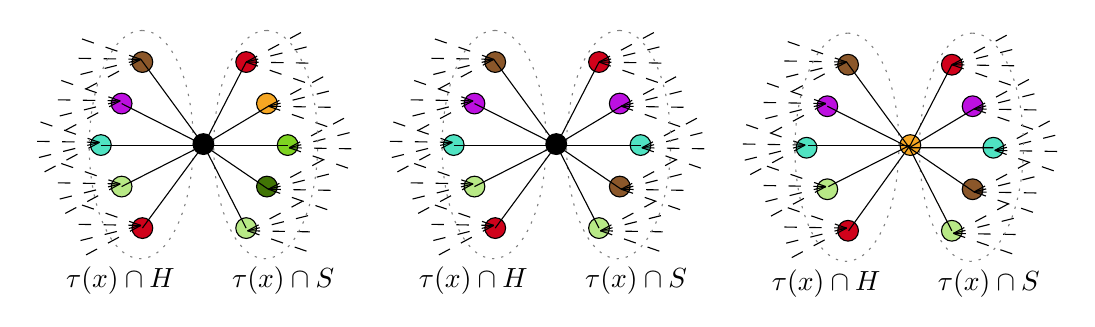
\begin{tikzpicture}[x=0.75pt,y=0.75pt,yscale=-1,xscale=1]
%uncomment if require: \path (0,300); %set diagram left start at 0, and has height of 300

%Flowchart: Connector [id:dp07782491532437497] 
\draw  [fill={rgb, 255:red, 139; green, 87; blue, 42 }  ,fill opacity=1 ] (100,105) .. controls (100,102.24) and (102.24,100) .. (105,100) .. controls (107.76,100) and (110,102.24) .. (110,105) .. controls (110,107.76) and (107.76,110) .. (105,110) .. controls (102.24,110) and (100,107.76) .. (100,105) -- cycle ;
%Flowchart: Connector [id:dp4349213418261434] 
\draw  [fill={rgb, 255:red, 189; green, 16; blue, 224 }  ,fill opacity=1 ] (90,125) .. controls (90,122.24) and (92.24,120) .. (95,120) .. controls (97.76,120) and (100,122.24) .. (100,125) .. controls (100,127.76) and (97.76,130) .. (95,130) .. controls (92.24,130) and (90,127.76) .. (90,125) -- cycle ;
%Flowchart: Connector [id:dp29242125182021317] 
\draw  [fill={rgb, 255:red, 80; green, 227; blue, 194 }  ,fill opacity=1 ] (80,145) .. controls (80,142.24) and (82.24,140) .. (85,140) .. controls (87.76,140) and (90,142.24) .. (90,145) .. controls (90,147.76) and (87.76,150) .. (85,150) .. controls (82.24,150) and (80,147.76) .. (80,145) -- cycle ;
%Flowchart: Connector [id:dp17955281693921343] 
\draw  [fill={rgb, 255:red, 184; green, 233; blue, 134 }  ,fill opacity=1 ] (90,165) .. controls (90,162.24) and (92.24,160) .. (95,160) .. controls (97.76,160) and (100,162.24) .. (100,165) .. controls (100,167.76) and (97.76,170) .. (95,170) .. controls (92.24,170) and (90,167.76) .. (90,165) -- cycle ;
%Flowchart: Connector [id:dp8283855233343105] 
\draw  [fill={rgb, 255:red, 208; green, 2; blue, 27 }  ,fill opacity=1 ] (100,185) .. controls (100,182.24) and (102.24,180) .. (105,180) .. controls (107.76,180) and (110,182.24) .. (110,185) .. controls (110,187.76) and (107.76,190) .. (105,190) .. controls (102.24,190) and (100,187.76) .. (100,185) -- cycle ;
%Flowchart: Connector [id:dp423941769601323] 
\draw  [fill={rgb, 255:red, 208; green, 2; blue, 27 }  ,fill opacity=1 ] (150,105) .. controls (150,102.24) and (152.24,100) .. (155,100) .. controls (157.76,100) and (160,102.24) .. (160,105) .. controls (160,107.76) and (157.76,110) .. (155,110) .. controls (152.24,110) and (150,107.76) .. (150,105) -- cycle ;
%Flowchart: Connector [id:dp15938991133945546] 
\draw  [fill={rgb, 255:red, 245; green, 166; blue, 35 }  ,fill opacity=1 ] (160,125) .. controls (160,122.24) and (162.24,120) .. (165,120) .. controls (167.76,120) and (170,122.24) .. (170,125) .. controls (170,127.76) and (167.76,130) .. (165,130) .. controls (162.24,130) and (160,127.76) .. (160,125) -- cycle ;
%Flowchart: Connector [id:dp46690683023426616] 
\draw  [fill={rgb, 255:red, 126; green, 211; blue, 33 }  ,fill opacity=1 ] (170,145) .. controls (170,142.24) and (172.24,140) .. (175,140) .. controls (177.76,140) and (180,142.24) .. (180,145) .. controls (180,147.76) and (177.76,150) .. (175,150) .. controls (172.24,150) and (170,147.76) .. (170,145) -- cycle ;
%Flowchart: Connector [id:dp41822494433321233] 
\draw  [fill={rgb, 255:red, 65; green, 117; blue, 5 }  ,fill opacity=1 ] (160,165) .. controls (160,162.24) and (162.24,160) .. (165,160) .. controls (167.76,160) and (170,162.24) .. (170,165) .. controls (170,167.76) and (167.76,170) .. (165,170) .. controls (162.24,170) and (160,167.76) .. (160,165) -- cycle ;
%Flowchart: Connector [id:dp9629224125308938] 
\draw  [fill={rgb, 255:red, 184; green, 233; blue, 134 }  ,fill opacity=1 ] (150,185) .. controls (150,182.24) and (152.24,180) .. (155,180) .. controls (157.76,180) and (160,182.24) .. (160,185) .. controls (160,187.76) and (157.76,190) .. (155,190) .. controls (152.24,190) and (150,187.76) .. (150,185) -- cycle ;
%Straight Lines [id:da7949746323623339] 
\draw  [dash pattern={on 4.5pt off 4.5pt}]  (155,105) -- (185.29,88.71) ;
%Straight Lines [id:da5155855657125827] 
\draw  [dash pattern={on 4.5pt off 4.5pt}]  (155,105) -- (189.29,96.43) ;
%Straight Lines [id:da43036442261927765] 
\draw  [dash pattern={on 4.5pt off 4.5pt}]  (155,105) -- (188.14,105.57) ;
%Straight Lines [id:da07167392392613647] 
\draw  [dash pattern={on 4.5pt off 4.5pt}]  (155,105) -- (183.86,115) ;
%Straight Lines [id:da4777118998680916] 
\draw  [dash pattern={on 4.5pt off 4.5pt}]  (165.71,126.29) -- (196,110) ;
%Straight Lines [id:da932211279377416] 
\draw  [dash pattern={on 4.5pt off 4.5pt}]  (165.71,126.29) -- (200,117.71) ;
%Straight Lines [id:da3156757748168697] 
\draw  [dash pattern={on 4.5pt off 4.5pt}]  (165.71,126.29) -- (198.86,126.86) ;
%Straight Lines [id:da4067851298827794] 
\draw  [dash pattern={on 4.5pt off 4.5pt}]  (165.71,126.29) -- (194.57,136.29) ;
%Straight Lines [id:da9811690031038591] 
\draw  [dash pattern={on 4.5pt off 4.5pt}]  (175.71,146.29) -- (206,130) ;
%Straight Lines [id:da8050148362052958] 
\draw  [dash pattern={on 4.5pt off 4.5pt}]  (175.71,146.29) -- (210,137.71) ;
%Straight Lines [id:da22357931039926282] 
\draw  [dash pattern={on 4.5pt off 4.5pt}]  (175.71,146.29) -- (208.86,146.86) ;
%Straight Lines [id:da34882444480714336] 
\draw  [dash pattern={on 4.5pt off 4.5pt}]  (175.71,146.29) -- (204.57,156.29) ;
%Straight Lines [id:da41540106661918574] 
\draw  [dash pattern={on 4.5pt off 4.5pt}]  (165.71,166.29) -- (196,150) ;
%Straight Lines [id:da9659299066448325] 
\draw  [dash pattern={on 4.5pt off 4.5pt}]  (165.71,166.29) -- (200,157.71) ;
%Straight Lines [id:da8406898052829679] 
\draw  [dash pattern={on 4.5pt off 4.5pt}]  (165.71,166.29) -- (198.86,166.86) ;
%Straight Lines [id:da7168775601655789] 
\draw  [dash pattern={on 4.5pt off 4.5pt}]  (165.71,166.29) -- (194.57,176.29) ;
%Straight Lines [id:da8159709648303738] 
\draw  [dash pattern={on 4.5pt off 4.5pt}]  (155.71,186.29) -- (186,170) ;
%Straight Lines [id:da8185439489406752] 
\draw  [dash pattern={on 4.5pt off 4.5pt}]  (155.71,186.29) -- (190,177.71) ;
%Straight Lines [id:da5671547576735302] 
\draw  [dash pattern={on 4.5pt off 4.5pt}]  (155.71,186.29) -- (188.86,186.86) ;
%Straight Lines [id:da5612350165005024] 
\draw  [dash pattern={on 4.5pt off 4.5pt}]  (155.71,186.29) -- (184.57,196.29) ;
%Straight Lines [id:da24030951376928134] 
\draw  [dash pattern={on 4.5pt off 4.5pt}]  (104.29,103.71) -- (74,120) ;
%Straight Lines [id:da3187860958940084] 
\draw  [dash pattern={on 4.5pt off 4.5pt}]  (104.29,103.71) -- (70,112.29) ;
%Straight Lines [id:da01708831951516221] 
\draw  [dash pattern={on 4.5pt off 4.5pt}]  (104.29,103.71) -- (71.14,103.14) ;
%Straight Lines [id:da036421584182044664] 
\draw  [dash pattern={on 4.5pt off 4.5pt}]  (104.29,103.71) -- (75.43,93.71) ;

%Straight Lines [id:da4545323697267918] 
\draw  [dash pattern={on 4.5pt off 4.5pt}]  (94.29,123.71) -- (64,140) ;
%Straight Lines [id:da2094951199837063] 
\draw  [dash pattern={on 4.5pt off 4.5pt}]  (94.29,123.71) -- (60,132.29) ;
%Straight Lines [id:da8799766808433833] 
\draw  [dash pattern={on 4.5pt off 4.5pt}]  (94.29,123.71) -- (61.14,123.14) ;
%Straight Lines [id:da9858256354991806] 
\draw  [dash pattern={on 4.5pt off 4.5pt}]  (94.29,123.71) -- (65.43,113.71) ;

%Straight Lines [id:da0869981652673667] 
\draw  [dash pattern={on 4.5pt off 4.5pt}]  (84.29,143.71) -- (54,160) ;
%Straight Lines [id:da5875768825862903] 
\draw  [dash pattern={on 4.5pt off 4.5pt}]  (84.29,143.71) -- (50,152.29) ;
%Straight Lines [id:da9981054979828283] 
\draw  [dash pattern={on 4.5pt off 4.5pt}]  (84.29,143.71) -- (51.14,143.14) ;
%Straight Lines [id:da28828513638152453] 
\draw  [dash pattern={on 4.5pt off 4.5pt}]  (84.29,143.71) -- (55.43,133.71) ;

%Straight Lines [id:da8756781078433081] 
\draw  [dash pattern={on 4.5pt off 4.5pt}]  (94.29,163.71) -- (64,180) ;
%Straight Lines [id:da4076097288292658] 
\draw  [dash pattern={on 4.5pt off 4.5pt}]  (94.29,163.71) -- (60,172.29) ;
%Straight Lines [id:da9067886144183188] 
\draw  [dash pattern={on 4.5pt off 4.5pt}]  (94.29,163.71) -- (61.14,163.14) ;
%Straight Lines [id:da8409330657503014] 
\draw  [dash pattern={on 4.5pt off 4.5pt}]  (94.29,163.71) -- (65.43,153.71) ;

%Straight Lines [id:da8790150296739412] 
\draw  [dash pattern={on 4.5pt off 4.5pt}]  (104.29,183.71) -- (74,200) ;
%Straight Lines [id:da8777752212862001] 
\draw  [dash pattern={on 4.5pt off 4.5pt}]  (104.29,183.71) -- (70,192.29) ;
%Straight Lines [id:da50676357983221] 
\draw  [dash pattern={on 4.5pt off 4.5pt}]  (104.29,183.71) -- (71.14,183.14) ;
%Straight Lines [id:da36710844709476154] 
\draw  [dash pattern={on 4.5pt off 4.5pt}]  (104.29,183.71) -- (75.43,173.71) ;

%Shape: Ellipse [id:dp35530944382621055] 
\draw  [color={rgb, 255:red, 128; green, 128; blue, 128 }  ,draw opacity=1 ][dash pattern={on 0.84pt off 2.51pt}] (104.96,89.77) .. controls (118.79,89.9) and (129.77,114.62) .. (129.49,145) .. controls (129.21,175.37) and (117.77,199.89) .. (103.94,199.76) .. controls (90.11,199.63) and (79.12,174.91) .. (79.4,144.53) .. controls (79.68,114.16) and (91.12,89.64) .. (104.96,89.77) -- cycle ;
%Shape: Ellipse [id:dp6849360838348542] 
\draw  [color={rgb, 255:red, 128; green, 128; blue, 128 }  ,draw opacity=1 ][dash pattern={on 0.84pt off 2.51pt}] (164.96,89.77) .. controls (178.79,89.9) and (189.77,114.62) .. (189.49,145) .. controls (189.21,175.37) and (177.77,199.89) .. (163.94,199.76) .. controls (150.11,199.63) and (139.12,174.91) .. (139.4,144.53) .. controls (139.68,114.16) and (151.12,89.64) .. (164.96,89.77) -- cycle ;
%Flowchart: Connector [id:dp8900095748728982] 
\draw  [fill={rgb, 255:red, 0; green, 0; blue, 0 }  ,fill opacity=1 ] (129.4,144.53) .. controls (129.4,141.77) and (131.64,139.53) .. (134.4,139.53) .. controls (137.16,139.53) and (139.4,141.77) .. (139.4,144.53) .. controls (139.4,147.29) and (137.16,149.53) .. (134.4,149.53) .. controls (131.64,149.53) and (129.4,147.29) .. (129.4,144.53) -- cycle ;
%Straight Lines [id:da2291696843657668] 
\draw    (104.29,103.71) -- (134.49,145) ;
%Straight Lines [id:da06032619749158896] 
\draw [fill={rgb, 255:red, 0; green, 0; blue, 0 }  ,fill opacity=1 ]   (134.49,145) -- (155,185) ;
%Straight Lines [id:da0959963213555024] 
\draw    (134.49,145) -- (165.71,166.29) ;
%Straight Lines [id:da8579554601468875] 
\draw    (134.49,145) -- (175,145) ;
%Straight Lines [id:da6333253136168397] 
\draw    (134.49,145) -- (165.71,126.29) ;
%Straight Lines [id:da1446351559236918] 
\draw    (134.49,145) -- (155,105) ;
%Straight Lines [id:da5799173300922372] 
\draw    (134.49,145) -- (105,185) ;
%Straight Lines [id:da5380918599859776] 
\draw    (134.49,145) -- (95,165) ;
%Straight Lines [id:da5983437417299301] 
\draw [fill={rgb, 255:red, 0; green, 0; blue, 0 }  ,fill opacity=1 ]   (134.49,145) -- (85,145) ;
%Straight Lines [id:da9072683806896357] 
\draw    (134.49,145) -- (95,125) ;
%Flowchart: Connector [id:dp4117919995882827] 
\draw  [fill={rgb, 255:red, 139; green, 87; blue, 42 }  ,fill opacity=1 ] (270,105) .. controls (270,102.24) and (272.24,100) .. (275,100) .. controls (277.76,100) and (280,102.24) .. (280,105) .. controls (280,107.76) and (277.76,110) .. (275,110) .. controls (272.24,110) and (270,107.76) .. (270,105) -- cycle ;
%Flowchart: Connector [id:dp3375255418407548] 
\draw  [fill={rgb, 255:red, 189; green, 16; blue, 224 }  ,fill opacity=1 ] (260,125) .. controls (260,122.24) and (262.24,120) .. (265,120) .. controls (267.76,120) and (270,122.24) .. (270,125) .. controls (270,127.76) and (267.76,130) .. (265,130) .. controls (262.24,130) and (260,127.76) .. (260,125) -- cycle ;
%Flowchart: Connector [id:dp5616954936846292] 
\draw  [fill={rgb, 255:red, 80; green, 227; blue, 194 }  ,fill opacity=1 ] (250,145) .. controls (250,142.24) and (252.24,140) .. (255,140) .. controls (257.76,140) and (260,142.24) .. (260,145) .. controls (260,147.76) and (257.76,150) .. (255,150) .. controls (252.24,150) and (250,147.76) .. (250,145) -- cycle ;
%Flowchart: Connector [id:dp6204871345789014] 
\draw  [fill={rgb, 255:red, 184; green, 233; blue, 134 }  ,fill opacity=1 ] (260,165) .. controls (260,162.24) and (262.24,160) .. (265,160) .. controls (267.76,160) and (270,162.24) .. (270,165) .. controls (270,167.76) and (267.76,170) .. (265,170) .. controls (262.24,170) and (260,167.76) .. (260,165) -- cycle ;
%Flowchart: Connector [id:dp49074867169534964] 
\draw  [fill={rgb, 255:red, 208; green, 2; blue, 27 }  ,fill opacity=1 ] (270,185) .. controls (270,182.24) and (272.24,180) .. (275,180) .. controls (277.76,180) and (280,182.24) .. (280,185) .. controls (280,187.76) and (277.76,190) .. (275,190) .. controls (272.24,190) and (270,187.76) .. (270,185) -- cycle ;
%Flowchart: Connector [id:dp5364577488301356] 
\draw  [fill={rgb, 255:red, 208; green, 2; blue, 27 }  ,fill opacity=1 ] (320,105) .. controls (320,102.24) and (322.24,100) .. (325,100) .. controls (327.76,100) and (330,102.24) .. (330,105) .. controls (330,107.76) and (327.76,110) .. (325,110) .. controls (322.24,110) and (320,107.76) .. (320,105) -- cycle ;
%Flowchart: Connector [id:dp810859067761758] 
\draw  [fill={rgb, 255:red, 189; green, 16; blue, 224 }  ,fill opacity=1 ] (330,125) .. controls (330,122.24) and (332.24,120) .. (335,120) .. controls (337.76,120) and (340,122.24) .. (340,125) .. controls (340,127.76) and (337.76,130) .. (335,130) .. controls (332.24,130) and (330,127.76) .. (330,125) -- cycle ;
%Flowchart: Connector [id:dp03171326594943147] 
\draw  [fill={rgb, 255:red, 80; green, 227; blue, 194 }  ,fill opacity=1 ] (340,145) .. controls (340,142.24) and (342.24,140) .. (345,140) .. controls (347.76,140) and (350,142.24) .. (350,145) .. controls (350,147.76) and (347.76,150) .. (345,150) .. controls (342.24,150) and (340,147.76) .. (340,145) -- cycle ;
%Flowchart: Connector [id:dp3531571208186408] 
\draw  [fill={rgb, 255:red, 139; green, 87; blue, 42 }  ,fill opacity=1 ] (330,165) .. controls (330,162.24) and (332.24,160) .. (335,160) .. controls (337.76,160) and (340,162.24) .. (340,165) .. controls (340,167.76) and (337.76,170) .. (335,170) .. controls (332.24,170) and (330,167.76) .. (330,165) -- cycle ;
%Flowchart: Connector [id:dp677177015892891] 
\draw  [fill={rgb, 255:red, 184; green, 233; blue, 134 }  ,fill opacity=1 ] (320,185) .. controls (320,182.24) and (322.24,180) .. (325,180) .. controls (327.76,180) and (330,182.24) .. (330,185) .. controls (330,187.76) and (327.76,190) .. (325,190) .. controls (322.24,190) and (320,187.76) .. (320,185) -- cycle ;
%Straight Lines [id:da5235583195815362] 
\draw  [dash pattern={on 4.5pt off 4.5pt}]  (325,105) -- (355.29,88.71) ;
%Straight Lines [id:da2536912075444535] 
\draw  [dash pattern={on 4.5pt off 4.5pt}]  (325,105) -- (359.29,96.43) ;
%Straight Lines [id:da23182990030884376] 
\draw  [dash pattern={on 4.5pt off 4.5pt}]  (325,105) -- (358.14,105.57) ;
%Straight Lines [id:da9268823282546476] 
\draw  [dash pattern={on 4.5pt off 4.5pt}]  (325,105) -- (353.86,115) ;
%Straight Lines [id:da5426579015787263] 
\draw  [dash pattern={on 4.5pt off 4.5pt}]  (335.71,126.29) -- (366,110) ;
%Straight Lines [id:da13183473097731946] 
\draw  [dash pattern={on 4.5pt off 4.5pt}]  (335.71,126.29) -- (370,117.71) ;
%Straight Lines [id:da4191752477721937] 
\draw  [dash pattern={on 4.5pt off 4.5pt}]  (335.71,126.29) -- (368.86,126.86) ;
%Straight Lines [id:da17034991713286407] 
\draw  [dash pattern={on 4.5pt off 4.5pt}]  (335.71,126.29) -- (364.57,136.29) ;
%Straight Lines [id:da2100898969367544] 
\draw  [dash pattern={on 4.5pt off 4.5pt}]  (345.71,146.29) -- (376,130) ;
%Straight Lines [id:da27006366446983343] 
\draw  [dash pattern={on 4.5pt off 4.5pt}]  (345.71,146.29) -- (380,137.71) ;
%Straight Lines [id:da2972662083717028] 
\draw  [dash pattern={on 4.5pt off 4.5pt}]  (345.71,146.29) -- (378.86,146.86) ;
%Straight Lines [id:da24146295357876646] 
\draw  [dash pattern={on 4.5pt off 4.5pt}]  (345.71,146.29) -- (374.57,156.29) ;
%Straight Lines [id:da2607376127684954] 
\draw  [dash pattern={on 4.5pt off 4.5pt}]  (335.71,166.29) -- (366,150) ;
%Straight Lines [id:da07542969791270049] 
\draw  [dash pattern={on 4.5pt off 4.5pt}]  (335.71,166.29) -- (370,157.71) ;
%Straight Lines [id:da4329707548353925] 
\draw  [dash pattern={on 4.5pt off 4.5pt}]  (335.71,166.29) -- (368.86,166.86) ;
%Straight Lines [id:da9294849473262563] 
\draw  [dash pattern={on 4.5pt off 4.5pt}]  (335.71,166.29) -- (364.57,176.29) ;
%Straight Lines [id:da4355889330101964] 
\draw  [dash pattern={on 4.5pt off 4.5pt}]  (325.71,186.29) -- (356,170) ;
%Straight Lines [id:da39364821193821287] 
\draw  [dash pattern={on 4.5pt off 4.5pt}]  (325.71,186.29) -- (360,177.71) ;
%Straight Lines [id:da8924585304934793] 
\draw  [dash pattern={on 4.5pt off 4.5pt}]  (325.71,186.29) -- (358.86,186.86) ;
%Straight Lines [id:da7349455546806467] 
\draw  [dash pattern={on 4.5pt off 4.5pt}]  (325.71,186.29) -- (354.57,196.29) ;
%Straight Lines [id:da7876274841604919] 
\draw  [dash pattern={on 4.5pt off 4.5pt}]  (274.29,103.71) -- (244,120) ;
%Straight Lines [id:da5744644468834686] 
\draw  [dash pattern={on 4.5pt off 4.5pt}]  (274.29,103.71) -- (240,112.29) ;
%Straight Lines [id:da993397359271426] 
\draw  [dash pattern={on 4.5pt off 4.5pt}]  (274.29,103.71) -- (241.14,103.14) ;
%Straight Lines [id:da37635718068837] 
\draw  [dash pattern={on 4.5pt off 4.5pt}]  (274.29,103.71) -- (245.43,93.71) ;

%Straight Lines [id:da8696929691027344] 
\draw  [dash pattern={on 4.5pt off 4.5pt}]  (264.29,123.71) -- (234,140) ;
%Straight Lines [id:da0703937572905804] 
\draw  [dash pattern={on 4.5pt off 4.5pt}]  (264.29,123.71) -- (230,132.29) ;
%Straight Lines [id:da6683887380763822] 
\draw  [dash pattern={on 4.5pt off 4.5pt}]  (264.29,123.71) -- (231.14,123.14) ;
%Straight Lines [id:da49589508415703354] 
\draw  [dash pattern={on 4.5pt off 4.5pt}]  (264.29,123.71) -- (235.43,113.71) ;

%Straight Lines [id:da3096159285854295] 
\draw  [dash pattern={on 4.5pt off 4.5pt}]  (254.29,143.71) -- (224,160) ;
%Straight Lines [id:da5869467331929314] 
\draw  [dash pattern={on 4.5pt off 4.5pt}]  (254.29,143.71) -- (220,152.29) ;
%Straight Lines [id:da9266935324217415] 
\draw  [dash pattern={on 4.5pt off 4.5pt}]  (254.29,143.71) -- (221.14,143.14) ;
%Straight Lines [id:da1481616876080838] 
\draw  [dash pattern={on 4.5pt off 4.5pt}]  (254.29,143.71) -- (225.43,133.71) ;

%Straight Lines [id:da5108595937035717] 
\draw  [dash pattern={on 4.5pt off 4.5pt}]  (264.29,163.71) -- (234,180) ;
%Straight Lines [id:da9371257378521323] 
\draw  [dash pattern={on 4.5pt off 4.5pt}]  (264.29,163.71) -- (230,172.29) ;
%Straight Lines [id:da5518012375446971] 
\draw  [dash pattern={on 4.5pt off 4.5pt}]  (264.29,163.71) -- (231.14,163.14) ;
%Straight Lines [id:da023923541215935096] 
\draw  [dash pattern={on 4.5pt off 4.5pt}]  (264.29,163.71) -- (235.43,153.71) ;

%Straight Lines [id:da5111330831894367] 
\draw  [dash pattern={on 4.5pt off 4.5pt}]  (274.29,183.71) -- (244,200) ;
%Straight Lines [id:da6201431222680114] 
\draw  [dash pattern={on 4.5pt off 4.5pt}]  (274.29,183.71) -- (240,192.29) ;
%Straight Lines [id:da7863742828375134] 
\draw  [dash pattern={on 4.5pt off 4.5pt}]  (274.29,183.71) -- (241.14,183.14) ;
%Straight Lines [id:da6547332328591293] 
\draw  [dash pattern={on 4.5pt off 4.5pt}]  (274.29,183.71) -- (245.43,173.71) ;

%Shape: Ellipse [id:dp4581218413715865] 
\draw  [color={rgb, 255:red, 128; green, 128; blue, 128 }  ,draw opacity=1 ][dash pattern={on 0.84pt off 2.51pt}] (274.96,89.77) .. controls (288.79,89.9) and (299.77,114.62) .. (299.49,145) .. controls (299.21,175.37) and (287.77,199.89) .. (273.94,199.76) .. controls (260.11,199.63) and (249.12,174.91) .. (249.4,144.53) .. controls (249.68,114.16) and (261.12,89.64) .. (274.96,89.77) -- cycle ;
%Shape: Ellipse [id:dp2374791440194447] 
\draw  [color={rgb, 255:red, 128; green, 128; blue, 128 }  ,draw opacity=1 ][dash pattern={on 0.84pt off 2.51pt}] (334.96,89.77) .. controls (348.79,89.9) and (359.77,114.62) .. (359.49,145) .. controls (359.21,175.37) and (347.77,199.89) .. (333.94,199.76) .. controls (320.11,199.63) and (309.12,174.91) .. (309.4,144.53) .. controls (309.68,114.16) and (321.12,89.64) .. (334.96,89.77) -- cycle ;
%Flowchart: Connector [id:dp32636521009294983] 
\draw  [fill={rgb, 255:red, 0; green, 0; blue, 0 }  ,fill opacity=1 ] (299.4,144.53) .. controls (299.4,141.77) and (301.64,139.53) .. (304.4,139.53) .. controls (307.16,139.53) and (309.4,141.77) .. (309.4,144.53) .. controls (309.4,147.29) and (307.16,149.53) .. (304.4,149.53) .. controls (301.64,149.53) and (299.4,147.29) .. (299.4,144.53) -- cycle ;
%Straight Lines [id:da2788527325655301] 
\draw    (274.29,103.71) -- (304.49,145) ;
%Straight Lines [id:da7683754466725521] 
\draw [fill={rgb, 255:red, 0; green, 0; blue, 0 }  ,fill opacity=1 ]   (304.49,145) -- (325,185) ;
%Straight Lines [id:da7438326741567215] 
\draw    (304.49,145) -- (335.71,166.29) ;
%Straight Lines [id:da07519734124780086] 
\draw    (304.49,145) -- (345,145) ;
%Straight Lines [id:da9953998010882452] 
\draw    (304.49,145) -- (335.71,126.29) ;
%Straight Lines [id:da9353539895576156] 
\draw    (304.49,145) -- (325,105) ;
%Straight Lines [id:da6714492599556577] 
\draw    (304.49,145) -- (275,185) ;
%Straight Lines [id:da7194866404076772] 
\draw    (304.49,145) -- (265,165) ;
%Straight Lines [id:da8516143707317884] 
\draw [fill={rgb, 255:red, 0; green, 0; blue, 0 }  ,fill opacity=1 ]   (304.49,145) -- (255,145) ;
%Straight Lines [id:da6664957873630569] 
\draw    (304.49,145) -- (265,125) ;
%Flowchart: Connector [id:dp3557655061999786] 
\draw  [fill={rgb, 255:red, 139; green, 87; blue, 42 }  ,fill opacity=1 ] (440,106.29) .. controls (440,103.52) and (442.24,101.29) .. (445,101.29) .. controls (447.76,101.29) and (450,103.52) .. (450,106.29) .. controls (450,109.05) and (447.76,111.29) .. (445,111.29) .. controls (442.24,111.29) and (440,109.05) .. (440,106.29) -- cycle ;
%Flowchart: Connector [id:dp48969123982633966] 
\draw  [fill={rgb, 255:red, 189; green, 16; blue, 224 }  ,fill opacity=1 ] (430,126.29) .. controls (430,123.52) and (432.24,121.29) .. (435,121.29) .. controls (437.76,121.29) and (440,123.52) .. (440,126.29) .. controls (440,129.05) and (437.76,131.29) .. (435,131.29) .. controls (432.24,131.29) and (430,129.05) .. (430,126.29) -- cycle ;
%Flowchart: Connector [id:dp7822311635219918] 
\draw  [fill={rgb, 255:red, 80; green, 227; blue, 194 }  ,fill opacity=1 ] (420,146.29) .. controls (420,143.52) and (422.24,141.29) .. (425,141.29) .. controls (427.76,141.29) and (430,143.52) .. (430,146.29) .. controls (430,149.05) and (427.76,151.29) .. (425,151.29) .. controls (422.24,151.29) and (420,149.05) .. (420,146.29) -- cycle ;
%Flowchart: Connector [id:dp8767693205512884] 
\draw  [fill={rgb, 255:red, 184; green, 233; blue, 134 }  ,fill opacity=1 ] (430,166.29) .. controls (430,163.52) and (432.24,161.29) .. (435,161.29) .. controls (437.76,161.29) and (440,163.52) .. (440,166.29) .. controls (440,169.05) and (437.76,171.29) .. (435,171.29) .. controls (432.24,171.29) and (430,169.05) .. (430,166.29) -- cycle ;
%Flowchart: Connector [id:dp7408451281382878] 
\draw  [fill={rgb, 255:red, 208; green, 2; blue, 27 }  ,fill opacity=1 ] (440,186.29) .. controls (440,183.52) and (442.24,181.29) .. (445,181.29) .. controls (447.76,181.29) and (450,183.52) .. (450,186.29) .. controls (450,189.05) and (447.76,191.29) .. (445,191.29) .. controls (442.24,191.29) and (440,189.05) .. (440,186.29) -- cycle ;
%Flowchart: Connector [id:dp7310738068155317] 
\draw  [fill={rgb, 255:red, 208; green, 2; blue, 27 }  ,fill opacity=1 ] (490,106.29) .. controls (490,103.52) and (492.24,101.29) .. (495,101.29) .. controls (497.76,101.29) and (500,103.52) .. (500,106.29) .. controls (500,109.05) and (497.76,111.29) .. (495,111.29) .. controls (492.24,111.29) and (490,109.05) .. (490,106.29) -- cycle ;
%Flowchart: Connector [id:dp11288914206423717] 
\draw  [fill={rgb, 255:red, 189; green, 16; blue, 224 }  ,fill opacity=1 ] (500,126.29) .. controls (500,123.52) and (502.24,121.29) .. (505,121.29) .. controls (507.76,121.29) and (510,123.52) .. (510,126.29) .. controls (510,129.05) and (507.76,131.29) .. (505,131.29) .. controls (502.24,131.29) and (500,129.05) .. (500,126.29) -- cycle ;
%Flowchart: Connector [id:dp03898760667119261] 
\draw  [fill={rgb, 255:red, 80; green, 227; blue, 194 }  ,fill opacity=1 ] (510,146.29) .. controls (510,143.52) and (512.24,141.29) .. (515,141.29) .. controls (517.76,141.29) and (520,143.52) .. (520,146.29) .. controls (520,149.05) and (517.76,151.29) .. (515,151.29) .. controls (512.24,151.29) and (510,149.05) .. (510,146.29) -- cycle ;
%Flowchart: Connector [id:dp16035699910309742] 
\draw  [fill={rgb, 255:red, 139; green, 87; blue, 42 }  ,fill opacity=1 ] (500,166.29) .. controls (500,163.52) and (502.24,161.29) .. (505,161.29) .. controls (507.76,161.29) and (510,163.52) .. (510,166.29) .. controls (510,169.05) and (507.76,171.29) .. (505,171.29) .. controls (502.24,171.29) and (500,169.05) .. (500,166.29) -- cycle ;
%Flowchart: Connector [id:dp37823929466229045] 
\draw  [fill={rgb, 255:red, 184; green, 233; blue, 134 }  ,fill opacity=1 ] (490,186.29) .. controls (490,183.52) and (492.24,181.29) .. (495,181.29) .. controls (497.76,181.29) and (500,183.52) .. (500,186.29) .. controls (500,189.05) and (497.76,191.29) .. (495,191.29) .. controls (492.24,191.29) and (490,189.05) .. (490,186.29) -- cycle ;
%Straight Lines [id:da22926651373306495] 
\draw  [dash pattern={on 4.5pt off 4.5pt}]  (495,106.29) -- (525.29,90) ;
%Straight Lines [id:da23785900258109516] 
\draw  [dash pattern={on 4.5pt off 4.5pt}]  (495,106.29) -- (529.29,97.71) ;
%Straight Lines [id:da1269575871383004] 
\draw  [dash pattern={on 4.5pt off 4.5pt}]  (495,106.29) -- (528.14,106.86) ;
%Straight Lines [id:da7025246163609957] 
\draw  [dash pattern={on 4.5pt off 4.5pt}]  (495,106.29) -- (523.86,116.29) ;
%Straight Lines [id:da2631945639221067] 
\draw  [dash pattern={on 4.5pt off 4.5pt}]  (505.71,127.57) -- (536,111.29) ;
%Straight Lines [id:da43610088606075403] 
\draw  [dash pattern={on 4.5pt off 4.5pt}]  (505.71,127.57) -- (540,119) ;
%Straight Lines [id:da14080675055365144] 
\draw  [dash pattern={on 4.5pt off 4.5pt}]  (505.71,127.57) -- (538.86,128.14) ;
%Straight Lines [id:da5966578017631272] 
\draw  [dash pattern={on 4.5pt off 4.5pt}]  (505.71,127.57) -- (534.57,137.57) ;
%Straight Lines [id:da06353959639406737] 
\draw  [dash pattern={on 4.5pt off 4.5pt}]  (515.71,147.57) -- (546,131.29) ;
%Straight Lines [id:da3085849424147663] 
\draw  [dash pattern={on 4.5pt off 4.5pt}]  (515.71,147.57) -- (550,139) ;
%Straight Lines [id:da972405301028814] 
\draw  [dash pattern={on 4.5pt off 4.5pt}]  (515.71,147.57) -- (548.86,148.14) ;
%Straight Lines [id:da536762393294252] 
\draw  [dash pattern={on 4.5pt off 4.5pt}]  (515.71,147.57) -- (544.57,157.57) ;
%Straight Lines [id:da6988909351467869] 
\draw  [dash pattern={on 4.5pt off 4.5pt}]  (505.71,167.57) -- (536,151.29) ;
%Straight Lines [id:da9754971708045939] 
\draw  [dash pattern={on 4.5pt off 4.5pt}]  (505.71,167.57) -- (540,159) ;
%Straight Lines [id:da3690488038698685] 
\draw  [dash pattern={on 4.5pt off 4.5pt}]  (505.71,167.57) -- (538.86,168.14) ;
%Straight Lines [id:da7639316773896808] 
\draw  [dash pattern={on 4.5pt off 4.5pt}]  (505.71,167.57) -- (534.57,177.57) ;
%Straight Lines [id:da1475160609512055] 
\draw  [dash pattern={on 4.5pt off 4.5pt}]  (495.71,187.57) -- (526,171.29) ;
%Straight Lines [id:da016603322626005612] 
\draw  [dash pattern={on 4.5pt off 4.5pt}]  (495.71,187.57) -- (530,179) ;
%Straight Lines [id:da4604790503527467] 
\draw  [dash pattern={on 4.5pt off 4.5pt}]  (495.71,187.57) -- (528.86,188.14) ;
%Straight Lines [id:da20917748276626835] 
\draw  [dash pattern={on 4.5pt off 4.5pt}]  (495.71,187.57) -- (524.57,197.57) ;
%Straight Lines [id:da3960454931860873] 
\draw  [dash pattern={on 4.5pt off 4.5pt}]  (444.29,105) -- (414,121.29) ;
%Straight Lines [id:da8424994835271623] 
\draw  [dash pattern={on 4.5pt off 4.5pt}]  (444.29,105) -- (410,113.57) ;
%Straight Lines [id:da8025407781048484] 
\draw  [dash pattern={on 4.5pt off 4.5pt}]  (444.29,105) -- (411.14,104.43) ;
%Straight Lines [id:da06172182115471048] 
\draw  [dash pattern={on 4.5pt off 4.5pt}]  (444.29,105) -- (415.43,95) ;

%Straight Lines [id:da5070218747754712] 
\draw  [dash pattern={on 4.5pt off 4.5pt}]  (434.29,125) -- (404,141.29) ;
%Straight Lines [id:da44267329926707144] 
\draw  [dash pattern={on 4.5pt off 4.5pt}]  (434.29,125) -- (400,133.57) ;
%Straight Lines [id:da6877855468818879] 
\draw  [dash pattern={on 4.5pt off 4.5pt}]  (434.29,125) -- (401.14,124.43) ;
%Straight Lines [id:da5879498373924557] 
\draw  [dash pattern={on 4.5pt off 4.5pt}]  (434.29,125) -- (405.43,115) ;

%Straight Lines [id:da28902313881543173] 
\draw  [dash pattern={on 4.5pt off 4.5pt}]  (424.29,145) -- (394,161.29) ;
%Straight Lines [id:da05286444542879831] 
\draw  [dash pattern={on 4.5pt off 4.5pt}]  (424.29,145) -- (390,153.57) ;
%Straight Lines [id:da8200403716090032] 
\draw  [dash pattern={on 4.5pt off 4.5pt}]  (424.29,145) -- (391.14,144.43) ;
%Straight Lines [id:da000605466611133143] 
\draw  [dash pattern={on 4.5pt off 4.5pt}]  (424.29,145) -- (395.43,135) ;

%Straight Lines [id:da9109994446832586] 
\draw  [dash pattern={on 4.5pt off 4.5pt}]  (434.29,165) -- (404,181.29) ;
%Straight Lines [id:da17043456146449576] 
\draw  [dash pattern={on 4.5pt off 4.5pt}]  (434.29,165) -- (400,173.57) ;
%Straight Lines [id:da4223162818208328] 
\draw  [dash pattern={on 4.5pt off 4.5pt}]  (434.29,165) -- (401.14,164.43) ;
%Straight Lines [id:da41609126490139736] 
\draw  [dash pattern={on 4.5pt off 4.5pt}]  (434.29,165) -- (405.43,155) ;

%Straight Lines [id:da27794861398616444] 
\draw  [dash pattern={on 4.5pt off 4.5pt}]  (444.29,185) -- (414,201.29) ;
%Straight Lines [id:da23706927762117724] 
\draw  [dash pattern={on 4.5pt off 4.5pt}]  (444.29,185) -- (410,193.57) ;
%Straight Lines [id:da6822108242500674] 
\draw  [dash pattern={on 4.5pt off 4.5pt}]  (444.29,185) -- (411.14,184.43) ;
%Straight Lines [id:da6987689129775486] 
\draw  [dash pattern={on 4.5pt off 4.5pt}]  (444.29,185) -- (415.43,175) ;

%Shape: Ellipse [id:dp2157508625529445] 
\draw  [color={rgb, 255:red, 128; green, 128; blue, 128 }  ,draw opacity=1 ][dash pattern={on 0.84pt off 2.51pt}] (444.96,91.05) .. controls (458.79,91.18) and (469.77,115.91) .. (469.49,146.28) .. controls (469.21,176.65) and (457.77,201.17) .. (443.94,201.04) .. controls (430.11,200.92) and (419.12,176.19) .. (419.4,145.82) .. controls (419.68,115.44) and (431.12,90.93) .. (444.96,91.05) -- cycle ;
%Shape: Ellipse [id:dp027282517207677492] 
\draw  [color={rgb, 255:red, 128; green, 128; blue, 128 }  ,draw opacity=1 ][dash pattern={on 0.84pt off 2.51pt}] (504.96,91.05) .. controls (518.79,91.18) and (529.77,115.91) .. (529.49,146.28) .. controls (529.21,176.65) and (517.77,201.17) .. (503.94,201.04) .. controls (490.11,200.92) and (479.12,176.19) .. (479.4,145.82) .. controls (479.68,115.44) and (491.12,90.93) .. (504.96,91.05) -- cycle ;
%Flowchart: Connector [id:dp23631893247509517] 
\draw  [fill={rgb, 255:red, 245; green, 166; blue, 35 }  ,fill opacity=1 ] (470,145) .. controls (470,142.24) and (472.24,140) .. (475,140) .. controls (477.76,140) and (480,142.24) .. (480,145) .. controls (480,147.76) and (477.76,150) .. (475,150) .. controls (472.24,150) and (470,147.76) .. (470,145) -- cycle ;
%Straight Lines [id:da36716907059683024] 
\draw    (444.29,105) -- (474.49,146.28) ;
%Straight Lines [id:da5092951370635599] 
\draw [fill={rgb, 255:red, 245; green, 166; blue, 35 }  ,fill opacity=1 ]   (474.49,146.28) -- (495,186.29) ;
%Straight Lines [id:da7118117756563062] 
\draw    (474.49,146.28) -- (505.71,167.57) ;
%Straight Lines [id:da9407841481895197] 
\draw    (474.49,146.28) -- (515,146.29) ;
%Straight Lines [id:da1766764296512341] 
\draw    (474.49,146.28) -- (505.71,127.57) ;
%Straight Lines [id:da16106524680497625] 
\draw    (475,145) -- (495,106.29) ;
%Straight Lines [id:da8442583194871953] 
\draw    (475,145) -- (435.51,165) ;
%Straight Lines [id:da868098343554372] 
\draw [fill={rgb, 255:red, 65; green, 117; blue, 5 }  ,fill opacity=1 ]   (475,145) -- (425.51,145) ;
%Straight Lines [id:da6849174031795032] 
\draw    (474.49,146.28) -- (435,126.29) ;
%Straight Lines [id:da7603908085191766] 
\draw    (475,145) -- (445.25,186.29) ;

% Text Node
\draw (67,202.4) node [anchor=north west][inner sep=0.75pt]    {$\tau ( x) \cap H$};
% Text Node
\draw (147,202.4) node [anchor=north west][inner sep=0.75pt]    {$\tau ( x) \cap S$};
% Text Node
\draw (237,202.4) node [anchor=north west][inner sep=0.75pt]    {$\tau ( x) \cap H$};
% Text Node
\draw (317,202.4) node [anchor=north west][inner sep=0.75pt]    {$\tau ( x) \cap S$};
% Text Node
\draw (407,203.69) node [anchor=north west][inner sep=0.75pt]    {$\tau ( x) \cap H$};
% Text Node
\draw (487,203.69) node [anchor=north west][inner sep=0.75pt]    {$\tau ( x) \cap S$};


\end{tikzpicture}\\
First we have the original setting for $H$ and $S$. Black is colour $d+1$. Then we recolour $S$. Finally we recolour $x$ with whatever colour we have left. 
\end{center}
(ii) \textit{I have solved this on a case by case basis but my intuition says there's a better way. I will update it when I find it.}


\end{document}